%%%%%%%%%%%%%%%%%%%%%%%%%%%%%%%%%%%%%%%%%%%%%%%%%%%%%%%%%%%%%%%%%%%%% 
%% This is a (brief) model paper using the achemso class 
%% The document class accepts keyval options, which should include 
%% the target journal and optionally the manuscript type. 
%%%%%%%%%%%%%%%%%%%%%%%%%%%%%%%%%%%%%%%%%%%%%%%%%%%%%%%%%%%%%%%%%%%%% 
\documentclass[journal=jpcbfk,manuscript=article]{achemso} 
 
%%%%%%%%%%%%%%%%%%%%%%%%%%%%%%%%%%%%%%%%%%%%%%%%%%%%%%%%%%%%%%%%%%%%% 
%% Place any additional packages needed here.  Only include packages 
%% which are essential, to avoid problems later. Do NOT use any 
%% packages which require e-TeX (for example etoolbox): the e-TeX 
%% extensions are not currently available on the ACS conversion 
%% servers. 
%%%%%%%%%%%%%%%%%%%%%%%%%%%%%%%%%%%%%%%%%%%%%%%%%%%%%%%%%%%%%%%%%%%%% 

%% Workaround for malfunctioning textsuperscript with pdfx and T1 encoding
\let\tmpa\textsuperscript
\DeclareTextCommandDefault{\textsuperscript}{\tmpa}

\usepackage[x11names]{xcolor}  % typesetting in color
%% Generate PDF/A-2u
%\usepackage[a-2u]{pdfx}
 
\usepackage[super]{natbib}         % citation style AUTHOR (YEAR), or AUTHOR [NUMBER]

\usepackage{achemso}  
\usepackage{rotating}  
%\usepackage{times} 
%\usepackage{lmodern}    %% Prefer Latin Modern fonts
\usepackage{graphicx} 
\usepackage{setspace} 
\usepackage{amsmath} 
\usepackage{epstopdf} 
\usepackage{csquotes} 
\usepackage{mhchem} 
\usepackage{chemfig} 
\usepackage[obeyFinal]{easy-todo}
\usepackage[english]{babel}
\usepackage{xr}
\externaldocument{manuscript}


\usepackage{subfig}
\usepackage{dcolumn}        % improved alignment of table columns
\usepackage{booktabs}       % improved horizontal lines in tables
\usepackage{paralist}       % improved enumerate and itemize

%% Character encoding: usually latin2, cp1250 or utf8:
\usepackage[utf8]{inputenc}
\usepackage[T1]{fontenc}

%\usepackage{markdown}  
 
%% The hyperref package for clickable links in PDF and also for storing
%% metadata to PDF (including the table of contents).
%% Most settings are pre-set by the pdfx package.
%\hypersetup{unicode}
%\hypersetup{breaklinks=true}
%\hypersetup{colorlinks,allcolors=DodgerBlue4}
 
%%%%%%%%%%%%%%%%%%%%%%%%%%%%%%%%%%%%%%%%%%%%%%%%%%%%%%%%%%%%%%%%%%%%% 
%% If issues arise when submitting your manuscript, you may want to 
%% un-comment the next line.  This provides information on the 
%% version of every file you have used. 
%%%%%%%%%%%%%%%%%%%%%%%%%%%%%%%%%%%%%%%%%%%%%%%%%%%%%%%%%%%%%%%%%%%%% 
%%\listfiles 
 
%%%%%%%%%%%%%%%%%%%%%%%%%%%%%%%%%%%%%%%%%%%%%%%%%%%%%%%%%%%%%%%%%%%%% 
%% Place any additional macros here.  Please use \newcommand* where 
%% possible, and avoid layout-changing macros (which are not used 
%% when typesetting). 
%%%%%%%%%%%%%%%%%%%%%%%%%%%%%%%%%%%%%%%%%%%%%%%%%%%%%%%%%%%%%%%%%%%%% 
\newcommand*\mycommand[1]{\texttt{\emph{#1}}} 
%%% Custom variables
% width suitable for fitting into a column in 1-column page layout
\newlength{\figwidth}
\setlength{\figwidth}{9 cm} 
\newlength{\figwidthsmall}
\setlength{\figwidthsmall}{6 cm} 
\newlength{\figwidthfull}
\setlength{\figwidthfull}{14 cm} 
\newlength{\figheightsmall}
\setlength{\figheightsmall}{6 cm} 
\newlength{\figheight}
\setlength{\figheight}{12 cm} 

 
%%%%%%%%%%%%%%%%%%%%%%%%%%%%%%%%%%%%%%%%%%%%%%%%%%%%%%%%%%%%%%%%%%%%% 
%% Meta-data block 
%% --------------- 
%% Each author should be given as a separate \author command. 
%% 
%% Corresponding authors should have an e-mail given after the author 
%% name as an \email command. Phone and fax numbers can be given 
%% using \phone and \fax, respectively; this information is optional. 
%% 
%% The affiliation of authors is given after the authors; each 
%% \affiliation command applies to all preceding authors not already 
%% assigned an affiliation. 
%% 
%% The affiliation takes an option argument for the short name.  This 
%% will typically be something like "University of Somewhere". 
%% 
%% The \altaffiliation macro should be used for new address, etc. 
%% On the other hand, \alsoaffiliation is used on a per author basis 
%% when authors are associated with multiple institutions. 
%%%%%%%%%%%%%%%%%%%%%%%%%%%%%%%%%%%%%%%%%%%%%%%%%%%%%%%%%%%%%%%%%%%%% 
 
\author{Josef Melcr} 
\email{melcr@marge.uochb.cas.cz} 
%%\homepage[]{https://jmelcr.github.io/}
\affiliation{Institute of Organic Chemistry and Biochemistry, 
Academy of Sciences of the Czech Republic,  
Prague 6, Czech Republic} 
\author{Pavel Jungwirth} 
%%\homepage[]{http://jungwirth.uochb.cas.cz/}
\affiliation{Institute of Organic Chemistry and Biochemistry, 
Academy of Sciences of the Czech Republic,  
Prague 6, Czech Republic} 
\alsoaffiliation{Department of Physics, Tampere University of Technology, P.O. Box 692, FI-33101 
Tampere, Finland} 
%SAMULI: We need to put tiago because the experimental acyl chain order parameters
\author{Tiago Ferreira}
\affiliation{Halle} 
\author{O. H. Samuli Ollila} 
\email{samuli.ollila@helsinki.fi} 
%%\homepage[]{Your web page} 
\affiliation{Institute of Organic Chemistry and Biochemistry, 
Academy of Sciences of the Czech Republic,  
Prague 6, Czech Republic} 
\alsoaffiliation{Institute of Biotechnology, University of Helsinki} 
 
 
%\author{Andrew N. Other} 
%\altaffiliation{A shared footnote} 
%\author{Fred T. Secondauthor} 
%\altaffiliation{Current address: Some other place, Othert\"own, 
%Germany} 
%\author{I. Ken Groupleader} 
%\altaffiliation{A shared footnote} 
%\email{i.k.groupleader@unknown.uu} 
%\phone{+123 (0)123 4445556} 
%\fax{+123 (0)123 4445557} 
%\affiliation[Unknown University] 
%{Department of Chemistry, Unknown University, Unknown Town} 
%\alsoaffiliation[Second University] 
%{Department of Chemistry, Second University, Nearby Town} 
%\author{Susanne K. Laborator} 
%\email{s.k.laborator@bigpharma.co} 
%\affiliation[BigPharma] 
%{Lead Discovery, BigPharma, Big Town, USA} 
%\author{Kay T. Finally} 
%\affiliation[Unknown University] 
%{Department of Chemistry, Unknown University, Unknown Town} 
%\alsoaffiliation[Second University] 
%{Department of Chemistry, Second University, Nearby Town} 
 
%%%%%%%%%%%%%%%%%%%%%%%%%%%%%%%%%%%%%%%%%%%%%%%%%%%%%%%%%%%%%%%%%%%%% 
%% The document title should be given as usual. Some journals require 
%% a running title from the author: this should be supplied as an 
%% optional argument to \title. 
%%%%%%%%%%%%%%%%%%%%%%%%%%%%%%%%%%%%%%%%%%%%%%%%%%%%%%%%%%%%%%%%%%%%% 
%\title[] 
%  {Accurate interactions of cations with 
%   neutral and negatively charged membranes 
%   via combination of experiments and molecular simulation}

%%SAMULI: new suggestion for the preliminary title
\title[] 
  { SUPPLEMENTARY INFORMATION: 
    Detailed structure of negatively charged membranes 
    of phosphatidylserine and phosphatidylcholine 
    at concentrations of calcium, sodium and potassium salts
    from molecular dynamics simulations with electronic polarization }

%%%%%%%%%%%%%%%%%%%%%%%%%%%%%%%%%%%%%%%%%%%%%%%%%%%%%%%%%%%%%%%%%%%%% 
%% Some journals require a list of abbreviations or keywords to be 
%% supplied. These should be set up here, and will be printed after 
%% the title and author information, if needed. 
%%%%%%%%%%%%%%%%%%%%%%%%%%%%%%%%%%%%%%%%%%%%%%%%%%%%%%%%%%%%%%%%%%%%% 
\abbreviations{IR,NMR,UV,MD,ECC,PC,PS,POPS,POPS} 
\keywords{MD simulation, molecular modeling, 
          polarizability, polarization,
          phospholipids, phosphatidylserine} 

%%%%%%%%%%%%%%%%%%%%%%%%%%%%%%%%%%%%%%%%%%%%%%%%%%%%%%%%%%%%%%%%%%%%% 
%% The manuscript does not need to include \maketitle, which is 
%% executed automatically. 
%%%%%%%%%%%%%%%%%%%%%%%%%%%%%%%%%%%%%%%%%%%%%%%%%%%%%%%%%%%%%%%%%%%%% 

\renewcommand{\thetable}{S\arabic{table}}%
\renewcommand{\thefigure}{S\arabic{figure}}%
\renewcommand{\thesection}{S\arabic{section}}%
\renewcommand{\thepage}{S\arabic{page}}%


\begin{document} 
 
\section{NMR experiments}
\begin{figure}[!h] 
  \centering 
  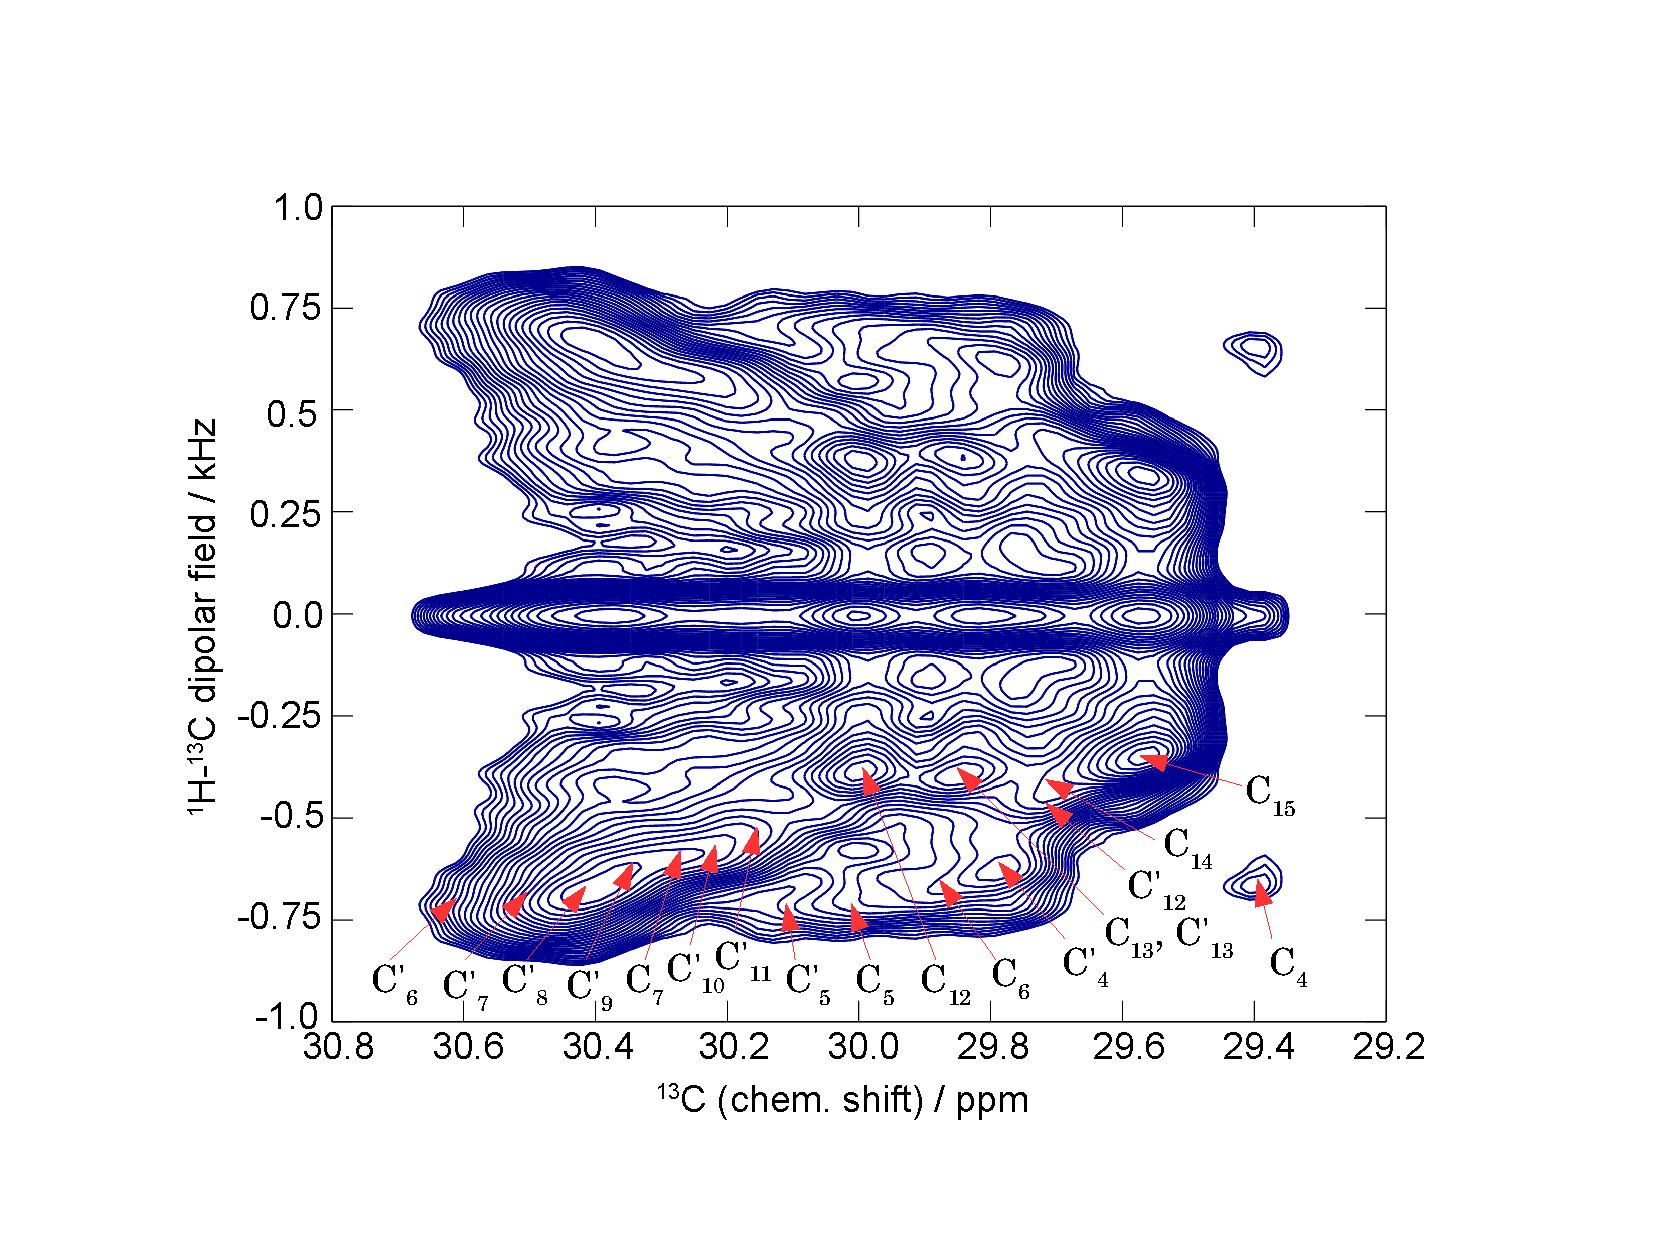
\includegraphics[width=\textwidth]{../Fig/crowded_region.pdf}
  \caption{\label{R-PDLF}
    2D-NMR R-PDLF spectra from the acyl chain region of POPS lipid bilayer.
  }
\end{figure}

\begin{figure}[hbp!] 
  \centering 
  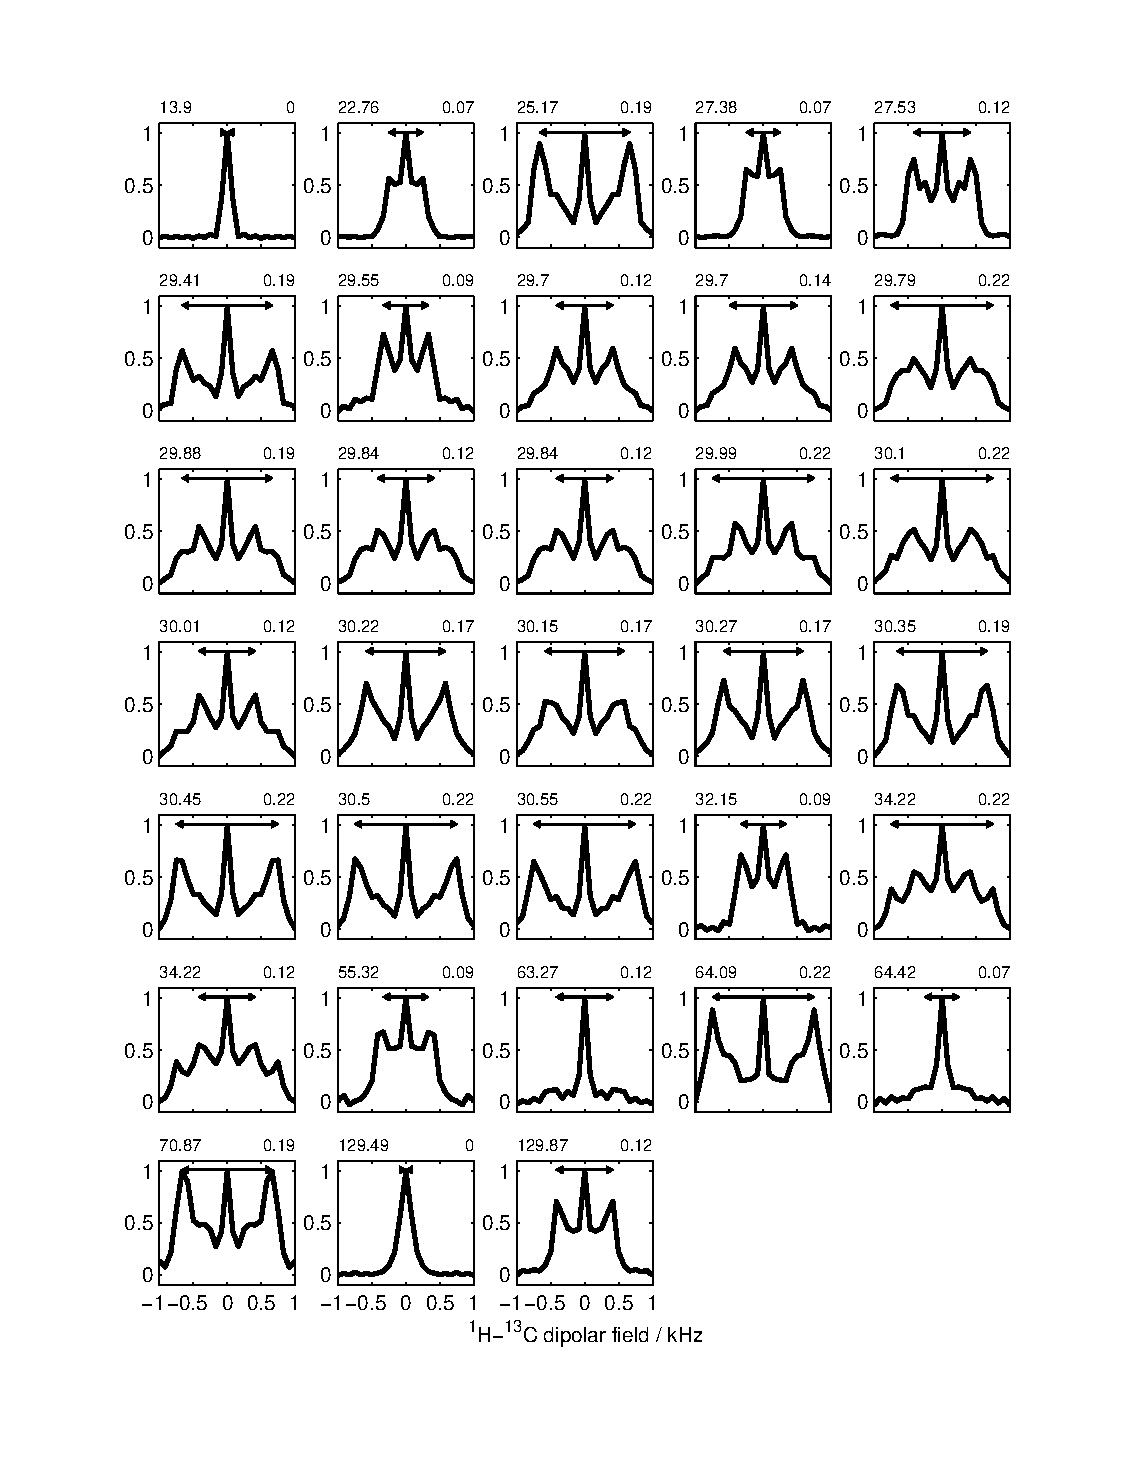
\includegraphics[width=\textwidth]{../Fig/slices_used.eps}
  \caption{\label{R-PDLFslices}
    Dipolar slices from the R-PDLF spectra used to determine the acyl chain order parameters of POPS.
  }
\end{figure} 



\pagebreak

\section{Distribution of dihedral angle \ce{C_\alpha-C_\beta-C_\gamma-O_\gamma} in POPS}
\begin{figure}[hbp!] 
  \centering 
  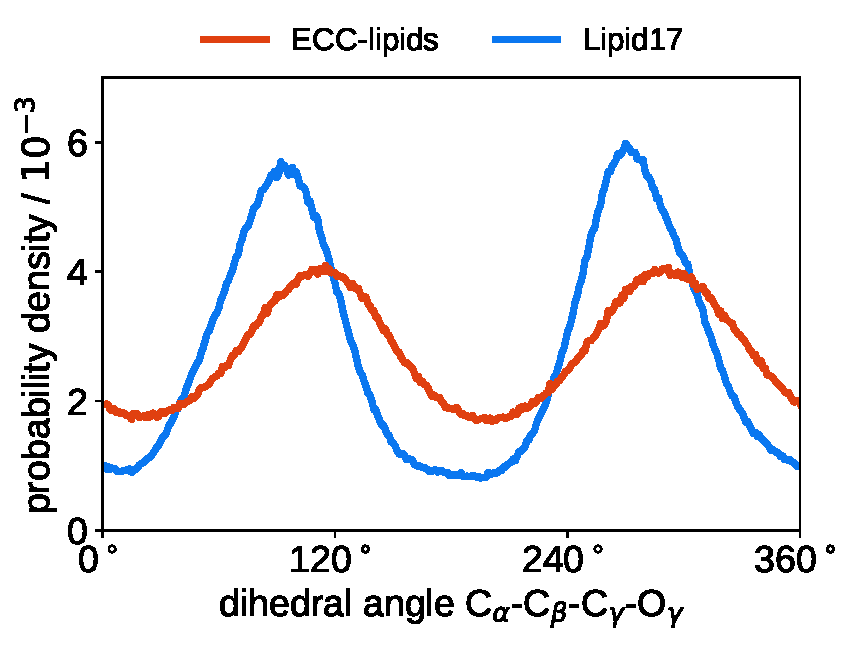
\includegraphics[width=\figwidth]{../img/dihedral_angle_distribution_Ca-Cb-Cg-Og_ECC-L17.pdf}
  \caption{\label{fig:dihedral}
    Distribution of dihedral angle \ce{C_\alpha-C_\beta-C_\gamma-O_\gamma} in POPS 
    from simulations of a pure POPS bilayer with \ce{Na+} counterions using Lipid17 and ECC-lipids. 
    Labelling of POPS segments is in Fig.~\ref{simVSexpNOions_POPS}. 
}
\todo{Cannot get rid of the copy of the Fig.1 cation}
\end{figure} 


\pagebreak
\section{Interactions of POPS with \ce{K+} and \ce{Na+} counterions and POPC}

\begin{figure}[hbp!] 
  \centering 
  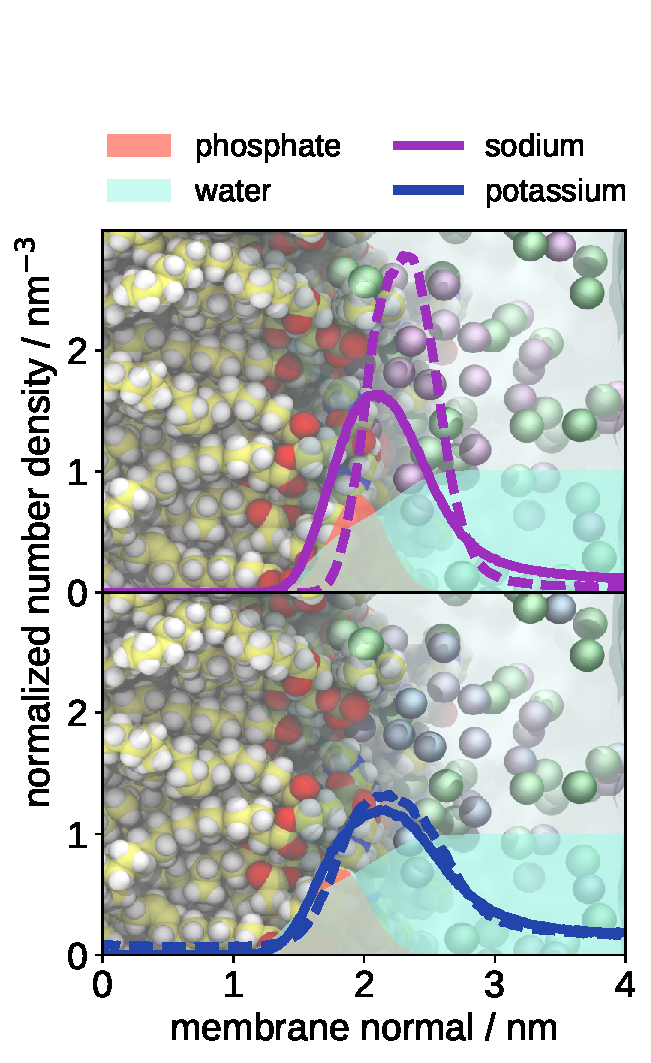
\includegraphics[height=\figheightsmall]{../img/ecc_pops/density_profiles_na-k-counterions_wat_phos_compar_purePOPS_ecclipids-lipid17.pdf}
  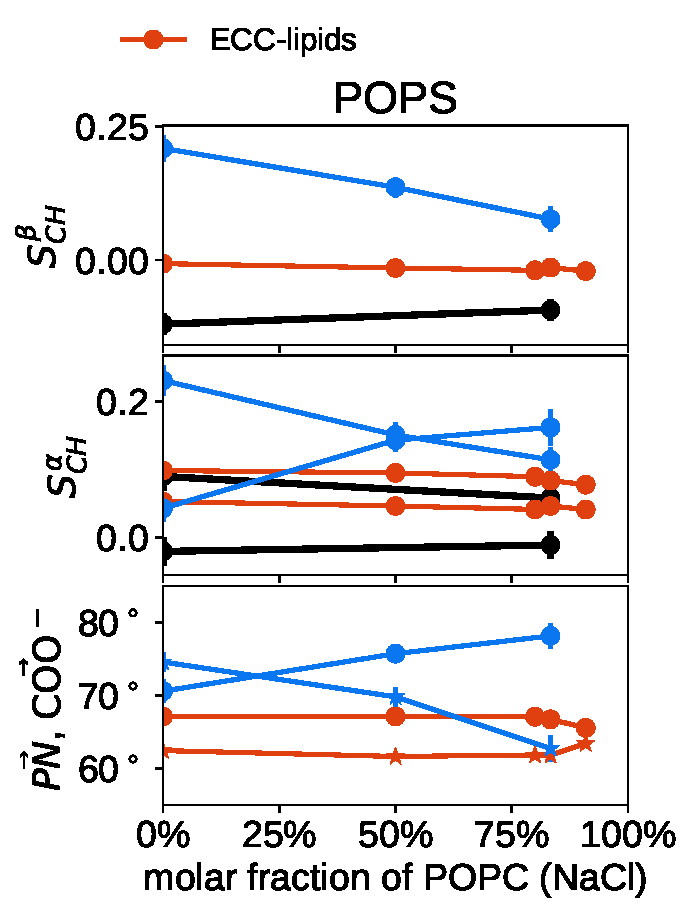
\includegraphics[height=\figheightsmall]{../Fig/order_parameters_changes_A-B_PC-PS_mix_POPS_nacl.pdf} 
  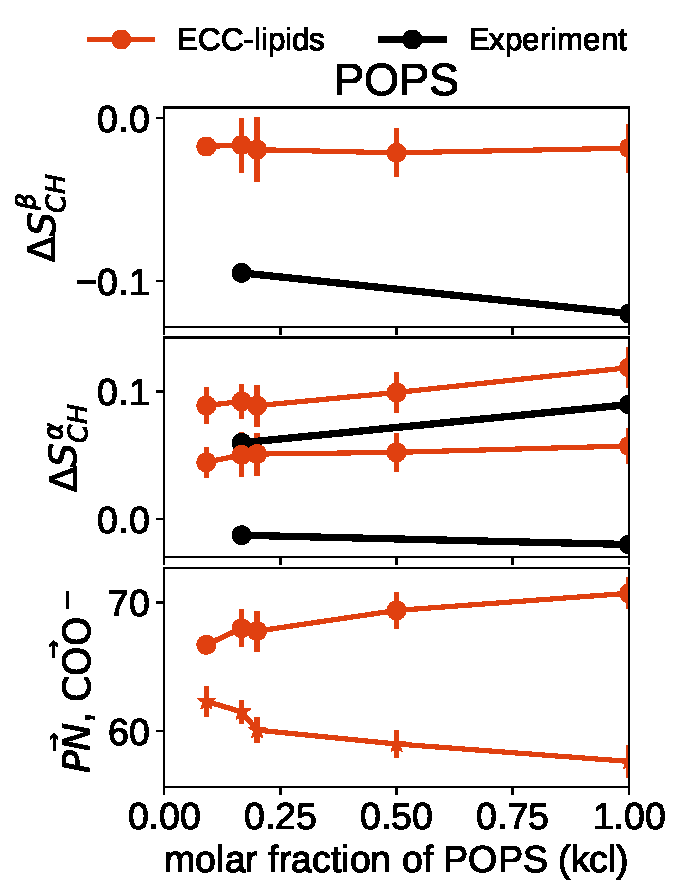
\includegraphics[height=\figheightsmall]{../Fig/order_parameters_changes_A-B_PC-PS_mix_POPS_kcl.pdf} 
  \caption{\label{fig:POPS-counterions-dens}
    \textbf{Left panel:} Number density profiles of \ce{K^{+}} and \ce{Na^{+}} counterions along the membrane normal axis
    in ECC-lipids (solid lines) and Lipid17/Dang (dashed lines) simulations of pure POPS bilayers.  
    The density profiles of phosphate groups and water are divided by 4 and 100, respectively.  
}
  \caption{\label{fig:delta_ordPar_NaCl_PC-PS_mix_PS} 
    \textbf{Right panels:} The POPS head group order parameters, the P--N and C$_\beta$--C$_\gamma$ vector angles (stars)
    with respect to the membrane normal as a function of POPC content in a bilayer
    from ECC-lipids and Lipid17/Dang simulations with \ce{Na^+} (left) and \ce{K^+} (right) counterions.
    Experimental order parameter values and signs for pure POPS are from Ref. \citenum{NMRlipidsIV} and values
    for POPC:POPS (5:1) mixture from Ref. \citenum{roux90} 
    (only \ce{Na^+} counterions, but shown also in the right plots for \ce{K+}).
    % No translation in y-axis done in this plot:
    %The underestimated response of ECC-lipids with \ce{Na^+} counterions 
    %is likely due to a still slightly overestimated binding affinity of \ce{Na^+} to the phospholipids,
    %which is corroborated by the series with \ce{K^+} counterions (lower affinity than \ce{Na^+}),
    %where the response is closer to the experiment, which uses only \ce{Na^+} counterions. 
  }
\end{figure} 



\pagebreak

\section{Density profiles of additional monovalent cations in POPC:POPS (5:1) mixtures}

\begin{figure}[!h] 
  \centering 
  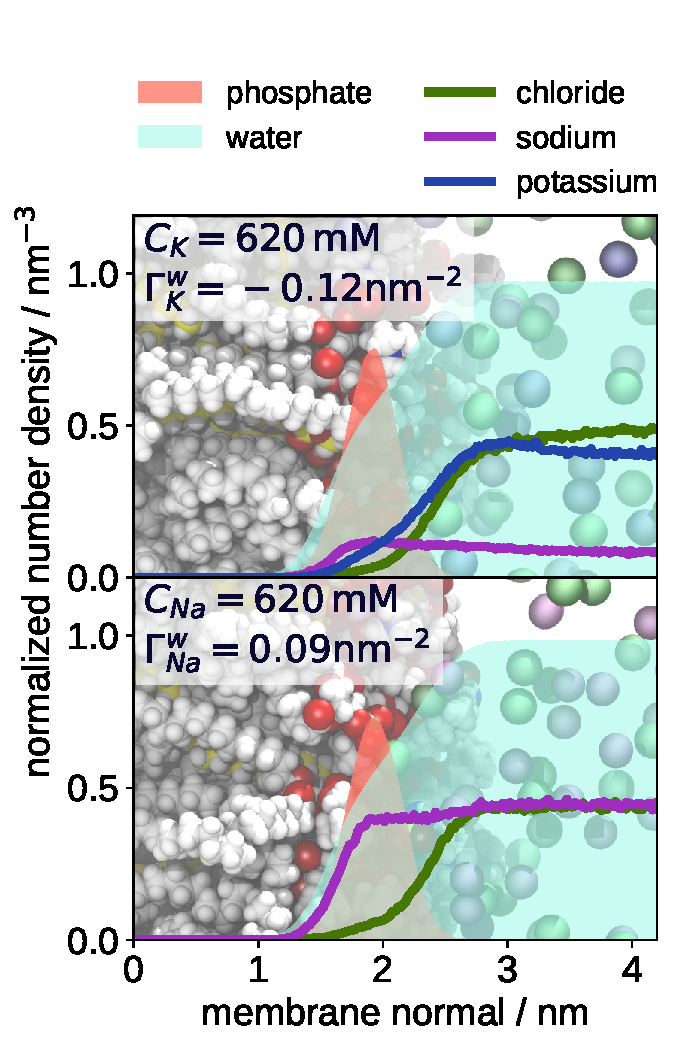
\includegraphics[width=\figwidth]{../img/ecc_pops/density_profiles_na_k_cl_wat_phos_models-compar_5-6_NaCl-and-KCl-series.pdf}
  \caption{\label{fig:nacl-dens_PCPS} 
    Number density profiles of \ce{K^{+}}, \ce{Na^{+}} and \ce{Cl^-} along the membrane normal axis
    from ECC-lipid simulation of POPC:POPS (5:1) mixture with \ce{Na^+} counterions and
    additional \ce{KCl} (top) and \ce{NaCl} (bottom) concentrations.
    The additional \ce{Na^+} are not distinguished from the counterions in bottom plot.
    The density profiles of phosphate groups and water are divided by 4 and 100, respectively.  
  }
\end{figure} 


\pagebreak
\section{Populations of bound \ce{Ca^{2+}} cations to the PC:PS (5:1) bilayer}

\begin{table}[h!] 
\centering
\caption{%Bulk concentrations, $C _{Ca}$, and buffer concentrations, $C' _{Ca}$, of Ca$^{2+}$;
  % relative surface excess of calcium with respect to water ($\Gamma_{Ca}^{\rm water}$); 
  % and
  Percentages of the population of bound Ca$^{2+}$ to various lipid moieties in a pure POPC bilayer with 350 mM CaCl$_2$
  and in a POPC:POPS (5:1) mixture with 409 mM CaCl$_2$. The threshold for counting a contact was set to $0.3\,\mathrm{nm}$, which encompasses the
  first peak of the radial distribution function between the cations and the oxygen atoms of the lipids. 
  \label{tab:binding}} 
\begin{tabular}{ l | c c } 
 exclusive interacting moiety &  \multicolumn{2}{c}{percentage of bound \ce{Ca^{2+}} } \\
%	\hline
%	$C _{Ca}\,/\,\mathrm{mM}$  &  $240\pm 10 $  &  $280\pm 10 $  \\
%	$C'_{Ca}\,/\,\mathrm{mM}$  &  $400\pm 10 $  &  $350\pm 10 $  \\
%	$\Gamma_{Ca}^{\rm water}\, / \,\mathrm{nm}^{-2}$  &  $0.24 \pm 0.01 $  &  $0.06 \pm 0.01 $  \\
%	\hline
%                             &  \multicolumn{2}{c}{ } \\
                             &  5\,POPC:1\,POPS &  POPC   \\
    \hline
    \textbf{PC}              &   59   &  100   \\
	     PO$_4$    in PC &   41   &   67   \\
	     carbonyls in PC &   <1   &   ~1   \\
    \hline
    \textbf{PS}              &    8   &        \\ 
	     PO$_4$  in PS   &    2   &        \\
	     COO$^-$ in PS   &    4   &        \\
	     carbonyls in PS &   <1   &        \\
    \hline
    \textbf{both PC and PS}  &   33   &        \\
      PC and PO$_4$  in PS   &    9   &        \\
      PC and COO$^-$ in PS   &   17   &        \\
      PC and carbonyls in PS &   <1   &        \\
  \end{tabular} \\
  %\todo{I have commented out the surface excess values (available in text) and concentrations (now in caption) from the table.} \\
  %\todo{I do not understand the numbers for different moieties. Are these probabilities that the calcium binds only to these moieties and
  %  nothing else? In total, 41 \% binds to PS lipids, but only 2 \% and 4 \% to phosphates and COO$^-$, respectively? Where do the rest bind?
  %  I think that we should show the total probabilities to bind to different moieties.}
\end{table} 


\pagebreak
\section{Residence times of cations}

%Timescales associated with the binding of calcium cations from solution to the membrane
%are plotted for each binding event as a histogram in Fig.~\ref{fig:hist_residence_times}. 
%
In ECC-lipid simulations, 90\% of the calcium residence times are shorter than $60\,\mathrm{ns}$ for pure POPC bilayer
and shorter than $200\,\mathrm{ns}$ for POPC:POPS (5:1) mixture, while the
longest observed residence times are $141\,\mathrm{ns}$ and $485\,\mathrm{ns}$, respectively (Fig.~\ref{fig:hist_residence_times}).
The significantly shorter residence times in ECC-lipid simulations than in simulations 
with other force fields~\cite{javanainen17, catte16} suggests that 1~$\mu$s simulations in this work
are sufficiently long to equlibrate the ion concentration on lipid bilayer interface.
%In summary, the results from ECC-lipids suggest 
%that the exchange of calcium between the POPC bilayer and the solvent 
%occurs at the order of $\sim$10--100~ns, 
%which is 
%Our results suggest that simulation trajectories with a characteristic length of several hundreds of nanoseconds 
%are necessary to capture the binding of calcium to neutral POPC bilayers 
%in equilibrium when more realistic \emph{polarizable} force fields are used. 
Interestingly, the calcium residence times are 3-4 times longer in POPC:POPS (5:1) mixture than in
pure POPC.

%Both estimates of the residence times come from simulations with comparable concentrations of around $250\mathrm{mM}$;
%the simulation with the neutral membrane has a bulk concentration of calcium $C_{ion} = 280\mathrm{mM}$, 
%whereas the simulation with the negatively charged membrane has a bulk concentration of calcium $C_{ion} = 240\mathrm{mM}$. 
%   In the simulation with the neutral membrane, 
%    90\% of the residence times of calcium cations are
%    shorter than $60\,\mathrm{ns}$, % exactly $53\,\mathrm{ns}$                                                                          
%    with the longest observed residence time being $141\,\mathrm{ns}$. 
%    In the simulation with the negatively charged membrane, 
%    90\% of the residence times of calcium cations are
%    shorter than $200\,\mathrm{ns}$, % exactly $53\,\mathrm{ns}$                                                                          
%    with the longest observed residence time being $485\,\mathrm{ns}$. 



\begin{figure}[!h]
  \centering
  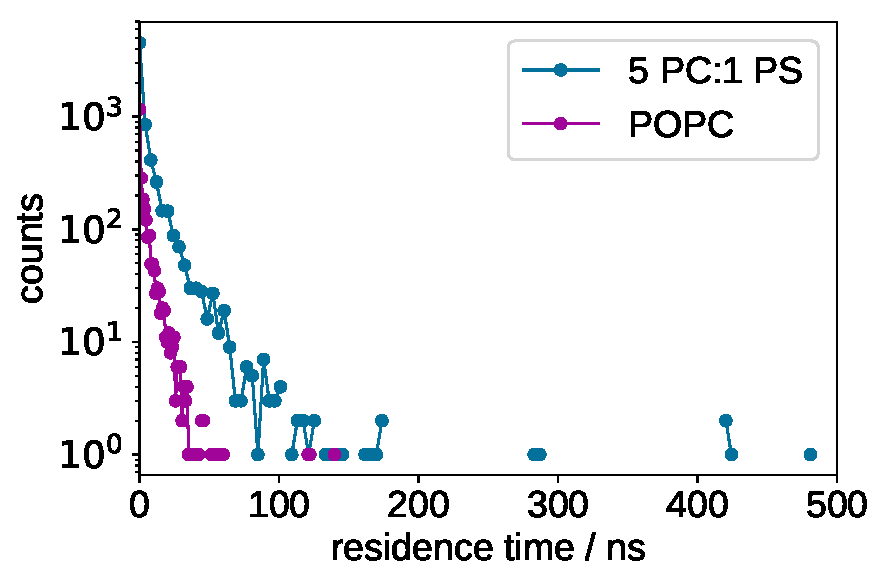
\includegraphics[width=\figwidth]{../img/histogram_bound_times_26CaCl2_comparison_PC-PCPS.pdf}
  \caption{\label{fig:hist_residence_times}
    Histograms of  \ce{Ca^{2+}} residence times in a pure POPC with 350 mM CaCl$_2$
    and in a POPC:POPS (5:1) mixture with 400 mM CaCl$_2$ from ECC-lipid simulations.
    %The simulation with the neutral membrane has a bulk concentration of calcium $C_{ion} = 280\mathrm{mM}$, 
    %the simulation with the negatively charged membrane has a bulk concentration of calcium $C_{ion} = 240\mathrm{mM}$. 
    Previously published simulation data \cite{melcr18} for pure POPC bilayers were taken directly from \cite{ECC-POPC_nacl_cacl2_files} Add Zenodo reference, if available. 
  }
\end{figure}



\bibliography{refs.bib} 
 
\end{document} 
 

